
%% bare_conf.tex
%% V1.3
%% 2007/01/11
%% by Michael Shell
%% See:
%% http://www.michaelshell.org/
%% for current contact information.
%%
%% This is a skeleton file demonstrating the use of IEEEtran.cls
%% (requires IEEEtran.cls version 1.7 or later) with an IEEE conference paper.
%%
%% Support sites:
%% http://www.michaelshell.org/tex/ieeetran/
%% http://www.ctan.org/tex-archive/macros/latex/contrib/IEEEtran/
%% and
%% http://www.ieee.org/

%%*************************************************************************
%% Legal Notice:
%% This code is offered as-is without any warranty either expressed or
%% implied; without even the implied warranty of MERCHANTABILITY or
%% FITNESS FOR A PARTICULAR PURPOSE! 
%% User assumes all risk.
%% In no event shall IEEE or any contributor to this code be liable for
%% any damages or losses, including, but not limited to, incidental,
%% consequential, or any other damages, resulting from the use or misuse
%% of any information contained here.
%%
%% All comments are the opinions of their respective authors and are not
%% necessarily endorsed by the IEEE.
%%
%% This work is distributed under the LaTeX Project Public License (LPPL)
%% ( http://www.latex-project.org/ ) version 1.3, and may be freely used,
%% distributed and modified. A copy of the LPPL, version 1.3, is included
%% in the base LaTeX documentation of all distributions of LaTeX released
%% 2003/12/01 or later.
%% Retain all contribution notices and credits.
%% ** Modified files should be clearly indicated as such, including  **
%% ** renaming them and changing author support contact information. **
%%
%% File list of work: IEEEtran.cls, IEEEtran_HOWTO.pdf, bare_adv.tex,
%%                    bare_conf.tex, bare_jrnl.tex, bare_jrnl_compsoc.tex
%%*************************************************************************
%

\documentclass[conference]{IEEEtran}

\usepackage{graphicx}
\usepackage{color}
\usepackage{multirow}
\usepackage{placeins}
\usepackage{mdwmath}

\newcommand \todo[1]{\textcolor{red}{\textsl{TODO: }}{\textcolor{black}{#1}}}
\newcommand \modified[1]{{\textcolor{black}{#1}}}
\hyphenation{op-tical net-works semi-conduc-tor}

\begin{document}
\title{Implementation and Evaluation of a PTP Transparent Clock Based on White Rabbit
Technology}
% author names and affiliations
% use a multiple column layout for up to three different
% affiliations
% 
% conference papers do not typically use \thanks and this command
% is locked out in conference mode. If really needed, such as for
% the acknowledgment of grants, issue a \IEEEoverridecommandlockouts
% after \documentclass

% for over three affiliations, or if they all won't fit within the width
% of the page, use this alternative format:
% 
\author{\IEEEauthorblockN{Cesar Prados\IEEEauthorrefmark{1}
\IEEEauthorrefmark{3}}
\IEEEauthorblockA{\IEEEauthorrefmark{1}GSI,Darmstadt Germany}
\IEEEauthorblockA{\IEEEauthorrefmark{3}Technical University Darmstadt, Darmstadt Germany}
}


\maketitle

\begin{abstract}
%\boldmath
White Rabbit is a new technology that allows to create an Ethernet timing network with
low-latency, deterministic packet delivery, sub-nanosecond accuracy and
picoseconds precision synchronization. WR is based on the  standards 
Synchronous Ethernet, IEEE 1588-2008 and PTP. 
Currently the synchronization of the clocks in the network is achieved 
by using WR Switches,  two-step Boundary Clocks (BC) using delay request-respond 
mechanism. In this paper, the author describes and evaluates the implementation  
of a WR Transparent Clock (TC) that uses the WR extension of PTP and is endowed with WR
hardware.
%Finally, we evaluate the suitability of the WR TCs in the Control and Timing
%System for the new Antiproton and Ion Research facility (FAIR) in GSI.
\end{abstract}




\section{Introduction}

Synchronization is one of the most important feature in control and timing
systems. The performance depends on the synchronization accuracy between 
the networking elements throughout the network, especially in systems 
where time-critical events are accurately scheduled to be executed in
distributed nodes. Such systems are quite common in particle accelerators
facilities, like the new timing system at GSI~\cite{biblio:FAIRtimingSystem} and 
CERN~\cite{biblio:cernWr}. The chosen technology  in both facilities is based on
the White Rabbit project. White Rabbit (WR) provides the technology and techniques to create a 
reliable and robust data and timing network with low-latency, deterministic packet 
delivery and synchronization. WR is based on the standards Synchronous Ethernet 
(SyncE)~\cite{biblio:synch} and  Ethernet (IEEE~802.3)~\cite{biblio:ethernet}. Besides, it extends IEEE~1588 
(PTP)~\cite{biblio:ptp} for achieving sub-nanoseconds  accuracy and picoseconds precision.
Besides GSI and CERN, in the WR project~\cite{biblio:wrproj} there are other 
institutes and experiments (LHAASO, KM3NeT etc...) that are taking an active part in 
development and adoption of the technology, as well as commercial companies (Seven Solutions, 
Integrasys, Elproma, Creotech, National Instruments etc..).

So far in WR, the synchronization is propagated in a hierarchical topology, from the master clock, 
WR Master (master), to the slave clocks, WR Slave (slave), using White Rabbit Switches (WRS). 
A WRS, in terms of PTP, is a two-step BC using the delay request-respond
mechanism (DDR) ~\cite{biblio:ptp}  
for the synchronization. In this paper, the author proposes an implementation
of a Transparent Clock (TC) using the existing WR extension to PTP, WRPTP~\cite{biblio:wrptp} 
and WR hardware~\cite{biblio:spec},~\cite{biblio:wrswitch}. 

Among the advantages of the Transparent Clocks (TC) for large timing networks
(e.g more than 2000 slaves in GSI), it is especially interesting
for the WR project the Peer-to-Peer TCs. They are suitable for timing
systems that require high resilience in the event of changes in the topology 
(e.g. switch failure), since the delay measurement is already available for
the synchronization in the new link, in contrast to Boundary Clocks (BC) that
have to calculate the delay once the new link is active. Another attractive feature 
of TCs for a WR timing system is the measurement of the residence time in the network 
devices which eliminates the error that results from queuing delays. 

In this paper, the author describes the WRPTP and WR synchronization (Section
II), and how the extension can be adopted by E2E and P2P TC (Section III). Then,
the author presents issues of implementing a WR TC  and an estimation of the performance.






\section{White Rabbit PTP}
\label{sec:wr}

\subsection{White Rabbit Synchronization}
WR reaches sub-nanosecond synchronization with  picoseconds jitter by
characterizing the asymmetries of the link and using a clock lookback
technique for tracking the phase shift between the master reference clock
signal and the looped back clock signal from the slave. In order to gather and
realize such measurements, WR extends PTP, WRPTP~\cite{biblio:ispcs_m}. 
Figure~\ref{fig:wr_ptp} shows the WRPTP flow of messages and the
integration with standard PTP once it is established .

Below, a resume of the steps, measurement and hardware support needed for the 
WR synchronization between two WR devices. A thoroughly description is presented 
in ~\cite{biblio:tomas} and ~\cite{biblio:wrptp}.

\subsubsection{WR Discovery and Syntonization}

A WR clock initiates WRPTP with an announcement message in order to discover
other WR devices. If a WR device has been discover the master will initiate the 
frequency lock procedure. WRPTP uses SyncE to distribute a common frequency throughout 
the network. The WR Slaves decodes the clock signal from the data stream sent
from the WR Master, and locks to it.

\subsubsection{Asymmetry Calibration}

Once the slave is locked to the master, the WR devices initiate to calibrate the 
asymmetries in the common optical link taking in consideration:

\begin{itemize}
    \item Fixed delays due to transmission circuitry
    \item Asymmetry of the optical transceivers and PHYs 
    \item Asymmetry of the propagation delay in the fiber caused by the chromatic dispersion
\end{itemize}

\subsubsection{Coarse and Fine Delay Measurement}

After the devices are calibrated, a first delay measurement, \textit{Coarse
Measurement}, is issued using the delay request-respond mechanism. 
The next step towards the synchronization requires the measurement of the phase shift
between a reference (master) clock signal and the looped-back clock signal
from  the slave, the \textit{round trip phase shift}, $phase_{mm}$. In Figure~\ref{fig:time_stamp}, 
the clock signal is looped back and the phase shift is measured 
using a phase detector, Digital Dual Mixer Time Difference (DDMTD) ~\cite{biblio:ddmtd}. With the
$phase_{mm}$, the delay round trip, $delay_{mm}$ is calculated. The $phase_{s}$
is the phase shift of the clock adjustment derived form the $offset_{ms}$. Using the 
$phase_{mm}$ and $phase_{s}$ the timestamps on ingress ports can be enhanced,
$t_{2p}$\footnote{The enhanced timestamps are distinguished from the
non-enhanced with a $p$} and  $t_{4p}$, using a decision algorithm described in ~\cite{biblio:tomas}.
Only timestamps on ingress ports need to be enhanced, since they are generated 
asynchronously to the reference clock domain. The \textit{Fine Delay Measurement}, round trip,
is calculated as follows using now the enhanced timestamps :

\begin{equation}
  \label{eq:round_trip}
    delay_{mm} = (t_{4p} - t_1) - (t_3 - t_{2p})
\end{equation}

\subsubsection{Synchronization}

In order to finish the synchronization, the offset between both clocks must be calculated, $offset_{mm}$. 
The round trip can be expressed as function of the  delay master to slave, $\sigma _{ms}$ , slave to
master $\sigma _{sm}$ and the sum of the fixed delays, $\Delta$ , obtained during the calibration.

\begin{equation}
  \label{eq:round_trip_2}
    delay_{mm} = \Delta + \sigma _{ms} + \sigma _{sm}
\end{equation}

The ratio between single delays is proportional to the asymmetry of the speed of
the different wavelengths due to the chromatic dispersion in the fiber optic
link:

\begin{equation}
    \label{eq:disp}
    (\alpha-1) = \frac{\sigma_{ms}}{\sigma_{sm}}
\end{equation}

Combining equations (\ref{eq:round_trip}), (\ref{eq:round_trip_2}) and
(\ref{eq:disp}), the delay master to slave and $offset_{MS}$:

\begin{equation}
    \label{eq:delayms}
     delay_{ms} = \frac{1+ \alpha}{2+ \alpha}(delay_{mm} - \Delta)+ \Delta_{txm} + \Delta_{rxs} 
\end{equation}

\begin{equation}
    \label{eq:offsetms}
    offset_{ms} = t_{1} - t_{2p} - delay_{ms}
\end{equation}


After the initial WRPTP synchronization, a DDR or Peer Delay mechanism produces the 
timestamps, $t_{1}$, $t_{2p}$, $t_{3}$ and $t_{4p}$ (in case Peer Delay, also
$t_{5}$ and $t_{6p})$ and the DDMTD tracks changes in the $phase_{mm}$ over time. 

\begin{figure}[!t]
\centering
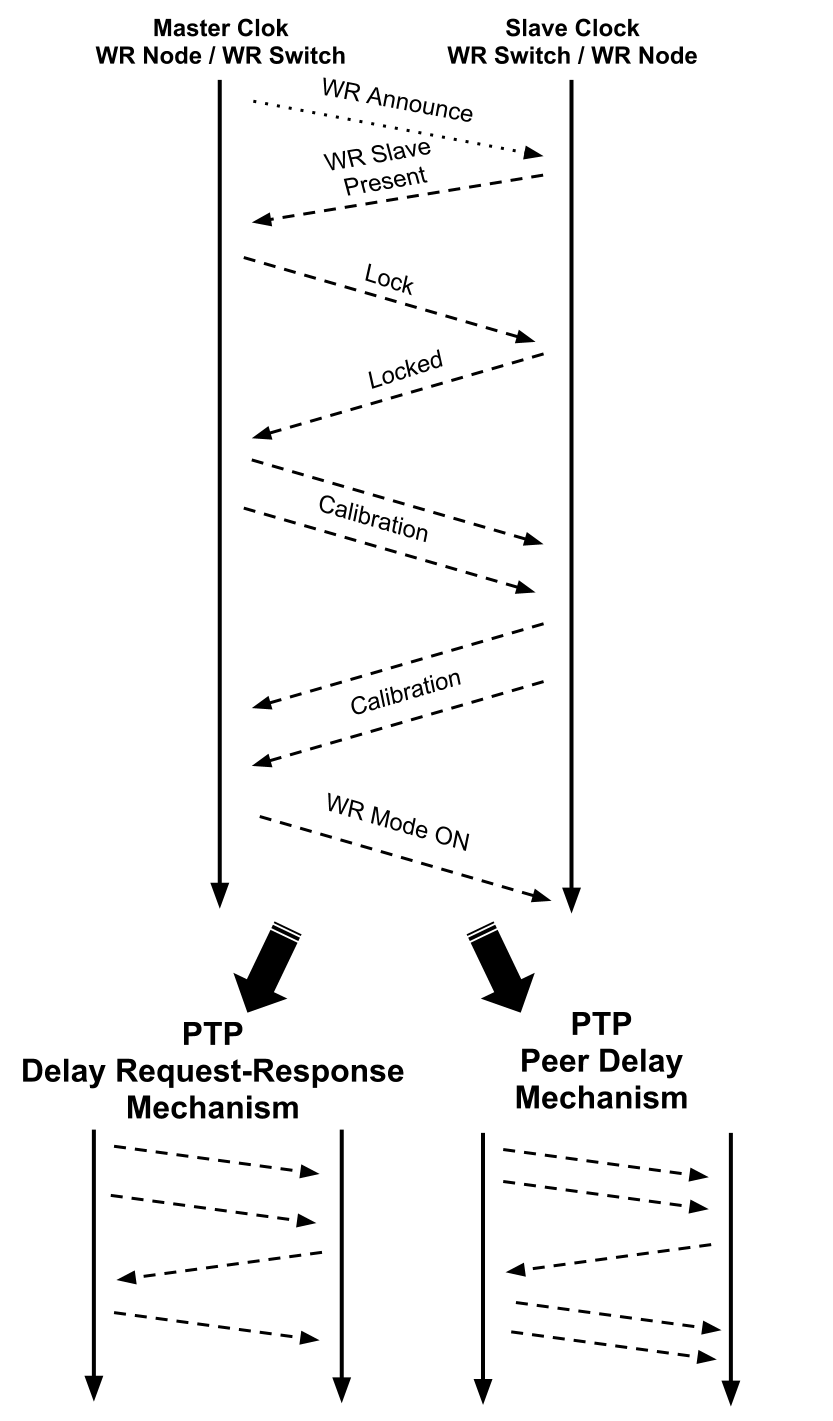
\includegraphics[scale=0.25]{fig/wr_ptp.png}
\caption{WR PTP Message Flow and PTP}
\label{fig:wr_ptp}
\end{figure}

%\FloatBarrier



\section{WR Transparent Clocks}
\label{sec:wr_tc}
PTP Transparent Clock (TC) modifies PTP messages as they pass through it
adding the residence time to the accumulative Correction Field (CF) in the PTP 
messages. Thus, the delay introduced  by the network is measured and can be 
subtracted in the slave clock, which improves distribution accuracy.

In section~\ref{sec:wr} the WRPTP and WR synchronization steps have been described for
master, slave and boundary clocks. In this chapter the author presents how a
standard TC becomes a WR TC.

\begin{figure*}[!t]
\centering
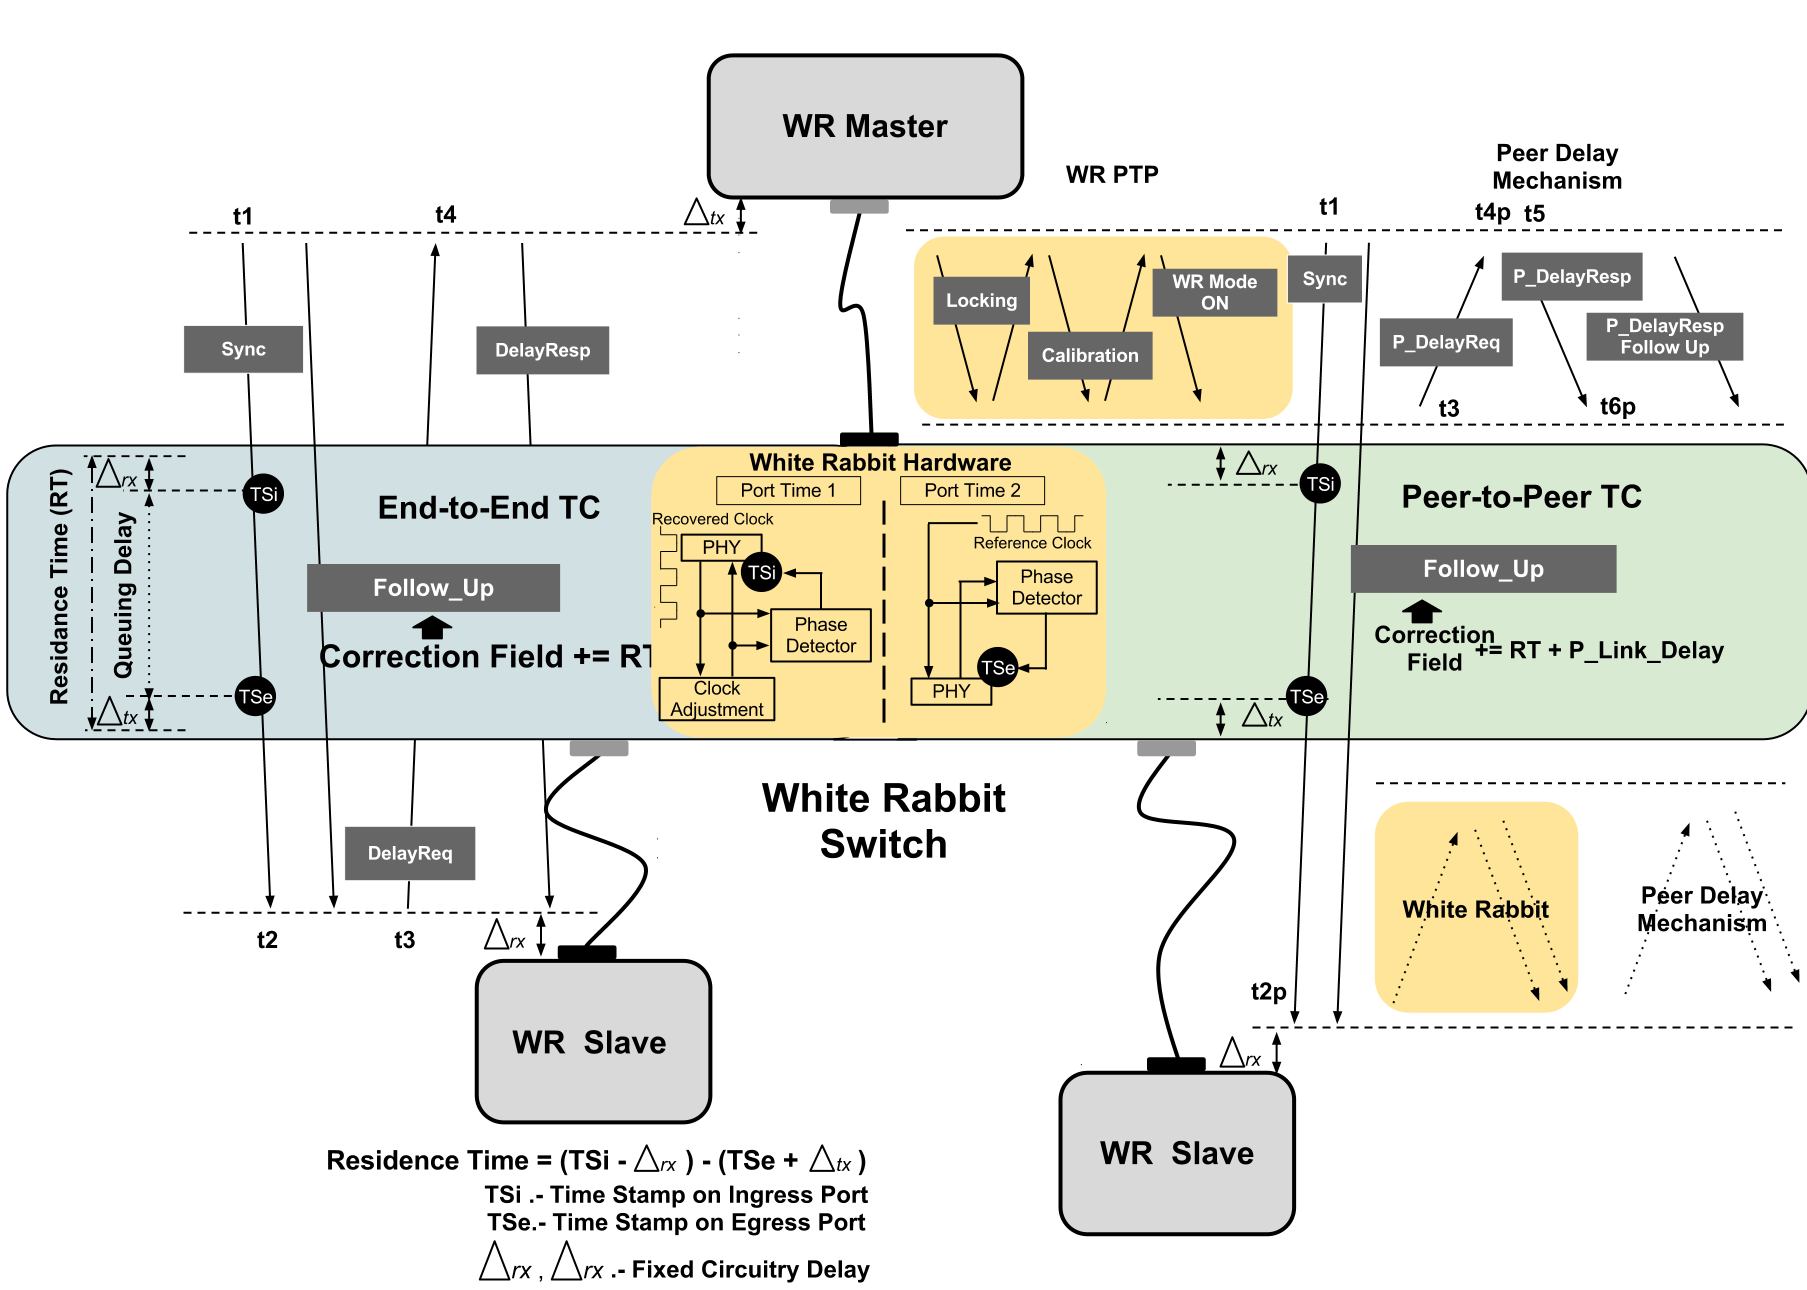
\includegraphics[scale=0.27]{fig/wr_schema_hw_bw.png}
\caption{WR E2E and P2P Transparent Clocks}
\label{fig:wr_tc}
\end{figure*}

\subsection{End-to-End WR Transparent Clock}

As in the standard, End-to-End (E2E) clocks, the WR E2E TC doesn't belong to the
master-slave hierarchy and doesn't synchronize to the WR Master. 
Therefore, a WR E2E accomplishes only the syntonization and the calibration,
the WR Mode is on, but there is no enhancement of the time stamps since the  
$delay_{ms}$ is calculated end to end, between master and slave, and there is 
not $phase_{mm}$ or $phase_{s}$ measurement. Thanks to the syntonization done 
during the WRPTP there is not errors in the 
measurement of the residence time.

Figure~\ref{fig:wr_tc} shows the PTP exchange of messages from master to slave,
going through the WRS transparently, and how the residence time is also calculated taking into 
account the fixed delays $\Delta$. A two-step WR E2E TC calculates, using
(\ref{eq:delayms}), the $offset_{ms}$:

\begin{equation}
    \label{eq:wre2e}
     CF += (TS_{ingress\_port} - \Delta_{rx}) -
     (TS_{egress\_port} + \Delta_{tx})
\end{equation}

\begin{equation}
    \label{eq:wre2e}
     offset_{ms} = t_{1} - t_{2} - delay_{ms} - CF
\end{equation}

\subsection{Peer-to-Peer WR Transparent Clock}

As the standard Peer-to-Peer (P2P) clocks, the WR P2P TC measures residence time
of Sync messages, and the link delay in both directions. Since the link delay
is done between adjacent clocks using the peer delay mechanism, the full WR synchronization
process can be issued between the two ports. The Figure~\ref{fig:wr_tc} shows how the
WR P2P initiates on after sides of the TC.

The measurement of the residence time, like in the E2E, are done without errors 
since the ports are syntonized to its master clock, but also the measurement of the
link delays, are as precise as the WR project claims~\cite{biblio:ispcs_m} for the
Boundary Clocks. The link delay is calculate like in (\ref{eq:delayms}) and the
Figure~\ref{fig:time_stamp} shows, but using $t_{3}$, $t_{4p}$, $t_{5}$ and
$t_{6p}$ instead. The $offset_{ms}$ is calculated :

\begin{equation}
    \label{eq:wre2e}
     CF += residance\_time + delay\_link
\end{equation}


\begin{equation}
    \label{eq:wre2e}
     offset_{ms}= t_{1} - t_{2} - CF - delay\_link\footnote{This link delay
     correspond to the las link to the slave}
\end{equation}



\FloatBarrier


\section{Implementation Issues and Performance Estimation}
\label{sec:issues}
The performance of a TC is commonly related to the ~\cite{biblio:tc_perf},
~\cite{biblio:tc_perf_2} following features: 

\begin{itemize}
    \item Timestamps accuracy 
    \item Correction factor stability
    \item Maximum update rate
    \item Rapid reconfiguration after topology changes
\end{itemize}

It applies to a WR TC as well.



WRS has been specially deceived to be compliant to most
common Ethernet standards (e.g. VLAN tags and Quality of Service) and fulfil demanding 
requirements in terms of upper-bound delivery, latency and fault tolerance. 
This features can be exploited to achieve remarkable performance as a TC.

\subsection{Time Stamping Accuracy}

In the chapter ~\ref{sec:wr}, the author resumes how WR accomplish
sub-nanoseconds synchronization and picoseconds jitter. It is based on the
characterization the asymmetries of the link a priory, and a clock lookback
technique. By doing this WR is able to  enhance the timestamps on ingress ports. 

The figure ~\ref{fig:time_stamp} shows that the Peer Delay timestamps between two 
adjacent nodes can be enhanced since the $pahse_{MM\_1}$ and $phase_{S\_1}$ to
the reference master clock signal are known. But it is not the case for $t_{2}$, 
this timestamp can be only enhanced using $phase_{S\_2}$ since the reference clock 
signal used in this link, is a synchronized clock to reference master clock signal 
(the same applies for $t_{4}$, in a E2E TC). The error introduced if the $t_{2}$ is 
enhanced using $phase_{S\_2}$ and not $phase_{S\_1}$ is:

x

x

x

x
Must be calculated!!!
x

x

x

\begin{figure*}[!t]
\centering
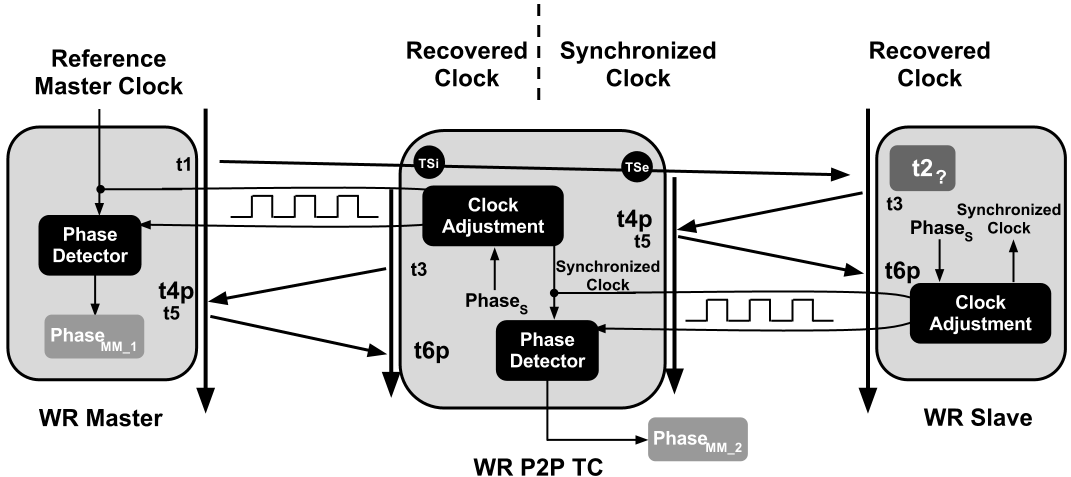
\includegraphics[scale=0.43]{fig/time_stamps_tc.png}
\caption{WR synchronization and P2P TC}
\label{fig:time_stamp}
\end{figure*}

\subsection{Correction Factor Stability and Maximum Update Rate}

Both, correction factor and  update rate, are features greatly influence
by the latency in the TC. As a result  synchronization could suffer
a degradation of the performance. An increment of the residence time in a TC normally is associated 
to increment of the traffic load handled by this TC. The authors of ~\cite{biblio:tc_perf} 
present the parameter \textit{Correction Factor Error} (CFE). It expresses the difference of the latency measured by a 
test equipment and the updated CF. The authors test TCs from different vendors
under high multicast load and compare the CFE result. 
The outcome of the test clarifies that switches with hardware treatment of the Sync messages 
maintain the CFE value low while the latency increases. Regarding
the WR TC, this is option that the  WRS enjoys already, hardware implementation 
of the timestamping unit, as well as hardware process forwarding of the Sync.

The \textit{Update Rate} (UR) for a two-step clock, is defined as the time between the transmission of a Sync
message from the master till the reception of the Follow Up message by the slave. 
High latencies, 10-30\% ~\cite{biblio:tc_perf} of the UR, can create 
instability in the slave. In addition, high latencies makes the TC no suitable for applications
demanding high UR. WRS is designed to provide low latency for time critical
information (e.g control accelerator information) using Cut-Through forwarding
schema and QoS \cite[vlan] in the output ports it is possible to queue the PTP
traffic in the second highest priority. By doing this the UR will be still high.

\FloatBarrier

\subsection{Reconfiguration after Topologies Changes}

The application of the timing system defines not only the requirements of accuracy, precision, 
but also the stability and continuation of the synchronization in the events
of(?) failure of TCs. The author doesn't (past/present??)
find references of this features for timing system based on PTP in the
literature. Nevertheless, the new timing system for GSI and CERN  have a demanding requirement
regarding the stability of the timing. 

TABLE

Both timing systems achieve resilience against network failures using redundant
topologies. Lowe layer protocols resolves the topology to a loop-free topologies. As
a result, the protocol sets port connected to cyclic paths to block/passive
state. In this case only the P2P TC still issues the synchronization between the
ports, and in both directions. As a result both clocks have the link delay
information. This offers the possibility of having immediately available the
link after change in the topology. It means that the reconfiguration time 
doesn't depend on TC anymore but in the  lower layer protocol. WRS has already a
proposals for implementing a transparent mechanism ~\cite{biblio:wrswitch} for
recovering from single points of failure in a redundant network.


%\section{FAIR and Transparent Clocks}
\label{sec:FAIR}


\subsection{Timing System Requirements}



\subsection{WR Network in FAIR Timing System}


\section{Conclusions and Future Work}


Conclusion-->>>






Currently the WR Switch V3 ~\cite{biblio:wrswitch} behaves as Boundary clock.
After an exhaustive examination of the WR project, the following features should be
added to the existing gateware and software (no modifications in the hardware)
for a proof of concept WR TC implementation:

\begin{itemize}
    \item Peer Delay Mechanism
    \item WR TC clock behaviour
    \item Hardware process of Sync and Follow Up messages
    \item Enhanced Timestamping across TC using WR
\end{itemize}

The openness of the project \footnote{The WRS is licensed under \textit{CERN Open Hardware Licence}
~\cite{biblio:lic}  and is publicly available in the Open Hardware Repository.},
plus the amount of work already done, makes the implementation achievable with a
reasonable effort.


\section{Acknowledgment}

The author would like to recognize the vast work done by the WR Community 
and thank specially to, T. W\l{}ostowski and M. Lipiński, for their support,  
design and code of the White Rabbit Switch, on which a I have based this paper.
I want also to thank to the timing team at GSI: D.Beck, M.Kreider, S.Rauch  and
W.Terpstra for the review and feedbacks of this paper.


\bibliographystyle{IEEEtran}
\bibliography{IEEEabrv,./biblio}

\end{document}


